\documentclass{VUMIFPSkursinis}
\usepackage{algorithmicx}
\usepackage{algorithm}
\usepackage{algpseudocode}
\usepackage{amsfonts}
\usepackage{amsmath}
\usepackage{bm}
\usepackage{caption}
\usepackage{color}
\usepackage{float}
\usepackage{graphicx}
\usepackage{listings}
\usepackage{subfig}
\usepackage{array}
\usepackage{wrapfig}
\usepackage{tabu}

% Titulinio aprašas
\university{Vilniaus universitetas}
\faculty{Matematikos ir informatikos fakultetas}
\department{Programų sistemų bakalauro studijų programa}
\papertype{Bakalauro baigiamasis darbas}
\title{Detalus vaizdų panašumas naudojant trejetų tinklus}
\titleineng{Fine-grained Images Similarity using Triplet-network}
\status{4 kurso 6 grupės studentas}
\author{Andrius Butkevičiuss}
% \secondauthor{Vardonis Pavardonis} % Pridėti antrą autorių
\supervisor{dr. Vytautas Valaitis}
\date{Vilnius – \the\year }

% Nustatymai
% \setmainfont{Palemonas} % Pakeisti teksto šriftą į Palemonas (turi būti įdiegtas sistemoje)
\bibliography{bibliografija}
\let\[\relax \let\]\relax % avoid warnings in the log file
\DeclareRobustCommand{\[}{\begin{equation}}
\DeclareRobustCommand{\]}{\end{equation}}
\begin{document}

\maketitle
\thispagestyle{empty} 

\tableofcontents

\sectionnonum{Padėka}
\thispagestyle{empty} 
Norėčiau padėkoti Vilniaus universiteto Matematikos ir Informatikos fakulteto dėstytojams už suteiktas žinias per šiuos keturis metus. Taip pat labai dėkoju savo dėstytojui, šio darbo vadovui, dr. Vytautui Valaičiui, už pagalbą ir patarimus šio bakalaurinio darbo metu.
\pagebreak

\sectionnonum{Santrauka}
\thispagestyle{empty} 
Šiame darbe yra aprašytas žmogaus siluetų vaizdų identifikavimas  naudojant trejetų tinklus. Šis modelis buvo pritaikytas apmokyti panaudojant CUHK01 ir Market-150 duomenų vaizdų rinkinius, rezultatai palyginti su kitais rinkoje esančiais tinklų modeliais. Išskirtos metrikos, pagal kurias rezultatai tarp modelių yra lyginami. Trejetų tinklas buvo panaudotas koreguojant populiarųjį VGG16 tinklų modelį,kuris yra paremtas konvoliucijomis. Šiam tiklui buvo pritaikyta naudoti trejetų nuostolių funkcija. Galiausiai buvo prietos išvados, kad norint identifikuoti to paties asmenes siluetus, trejetų tinklų modelis gali būti taikomas praktikoje, nes sugeba fiksuoti santykinai gerus rezultatus, kurie gali perspektyviai varžytis su kitų rinkoje esančių tinklų pasiektais rezultatais identifikuojant žmonių siluetus.
\newline
\textbf{Raktiniai žodžiai: konvoliuciniai neuroniai tinklai, trejetų nuostolių funkcija, nueroninių tinklų mokymas.}
\pagebreak

\sectionnonum{Summary}
\thispagestyle{empty} 
This work describes person re-identification by using Triplet-network model implementation. It was trained by using several datasets - CUHK01 and Market-150. The final results were compared with other competitive image recognition networks in a market. In order to have correct comparison results some metrics were provided. Triplet-network was achieved by customizing one of the most popular  pre-trained convolutional neural networks - VGG16. Instead of using traditional loss function - triplet loss function was used. After comparing the produced final results with other networks data results, the conclusion was reached that triplet networks can be considered as strongly competitive network because it cab reache great identification accuracy after it is trained with datasets mentioned previously.
\newline
\textbf{Key words: convolutional neural networks, re-identification, triplet loss function, neural network training.}
\pagebreak

\sectionnonum{Įvadas}

\thispagestyle{empty} 
Vaizdų tarpusavio panašumo identifikavimas tampa plačiai taikomas bei susilaukia vis daugiau dėmesio informacinių technologijų srityje. Viena iš to priežasčių - populiarėjant nuotolinių būdų prieinamiems vaizdams, atsiranda didesnė paklausa, kaip šiuos duomenis efektyviau atpažinti įvairiuose srityse. Taip pat, puikūs pasiekti rezultatai pasitelkiant giliuosius konvoliucinius neuroninius tinklus bei galimybė juos apmokyti didžiuliais duomenų rinkiniais, leidžia susilaukti vis didesnio dėmesio rinkoje. Visgi, siekiant atpažinti vaizdus tarpusavyje ir išgauti kuo korektiškesnius rezultatus yra susiduriama su problemomis. Kompiuteriui nėra lengva atskirti vizualius skirtumus ir objektų bruožų panašumus lengvai, kaip palyginus žmogui, kuris gali akimirskniu sugebėti atpažinti aplink jį esamus objektus. Kompiuteriui tą atlikti reikalauja daug resursų ir tam įvykdyti yra pasitelkiama daug matematinių operacijų. Tačiau atsirandantys nauji algoritmai, padedantys efektyviau atpažinti vizualius objektų skirtumus, leidžia konkuruoti vaizdų atpažinime su žmogumi. Šiuo metu vaizdų identifikavimas ar jų palyginimas tarpusavyje yra plačiai taikomas įvairiose sritye, pvz.: vaizdinės tapatybės nustatymui, veidų atpažinimui, esamos vietovės aptikimui pasitelkient beipiločiais orlaiviais užfiksuotas žemės reljefo nuotraukas ar reikiamų vaizdų suradimui pasitelkiant paieškos sistemas. Norint sugebėti tai atpažinti ir klasifikuoti, yra pasitelkiami įvairūs perspektyvūs tinklų modeliai ir algortimai, jie apmokami vaizdams atpažinti. Tam yra panaudojami konvoliuciniai tinklų modeliai, kurie išgauna puikius rezultatus. Vieni iš tokių tinklų -  Siamo arba trejetų tinklai. Šie tinklai susideda iš dviejų ar trijų vienodų ir lygiagrečių konvoliucinių neuronų tinkle esančių atšakų, kurios tarpusavyje dalinasi svoriais, kurių dėka galima gauti aukšto lygio nuotraukų bruožų atvaizdavimą taip leidžiant panašioms nuotraukoms būti kuo arčiau sujungtoms viena su kita funkcijos erdvėje. Tuo metu nepanašiems vaizdams – būnant atitolusiems toliau nuo teisingų nuotraukų. 
\newline	
Rinkoje yra siūlomi įvairūs konvoliucinių neuronų tinklų modeliai, pvz.: Alexnet, VGGNet, GoogLetNet, ResNet \cite{Aerial_image_similarity}. Verta paminėti, kad visi šie modeliai turėjo efektyvius atpažinimo rezultatus ILSVRC. Vis dažniau yra pasitelkiama prieš tai minėti trejetų tinklai, kurie optimizuoja bruožų atstumus erdvėje. Visgi sudėtingiausia problema išlieka semantinio tarpo problema, kuri atsiranda tarp žemos rezoliucijos nuotraukos pikselių užfiksuotų kompiuterinių sistemų ir aukšo lygio semantinių konceptų, kurias suvokia žmonės. Dėl to reikia rasti geresnių būdų, kaip sugebėti pateikti nuotrauką kompiuteriui ir gauti gilesnias jos semantinius bruožus. 
\newline
Todėl šio darbo tikslas yra pasiūlyti pasirinktą trejetų tinklų modelį \cite{Aerial_image_similarity}, kuris sugebėtų atpažinti žmonių siluetus su pasirinktais duomenų rinkiniais. Palyginti pasirinktą modelį su kitais esamais rinkoje modeliais, palyginti rezultatus. Taip pat išskirti metrikas tam. Išsiaiškinti su kuriais konkrečiais vaizdais pasirinktas modelis prastai fiksuodavo atpažinimą, įvardinti to priežastis.
\pagebreak
 
\textbf{Darbo tikslas} yra apmokyti trejetų tinklų modelį atpažinti to paties asmens silutetus nuotraukose, rezultatus palyginti su kitais tinklų modeliais. Todėl tikslui pasiekti reikia atlikti \textbf{šiuos uždavinius}:
\begin{enumerate}
\item{Išsinagrinėti literatūrą apie trejetų tinklų modelį}
\item{Išskirti metrikas pagal kurias galėtų analizuoti gautus rezultatus, panaudojant trejetų tinklų modelį.}
\item{Pasiūlyti pasirinktą trejetų tinklų modelį bei atpažinti vaizdų panašumus iš pasirinkto duomenų rinkinio.}
\item{Įvertinti modelio rezultatus}
\item{Pagal išskirtas metrikas palyginti rezultatus su kitais rinkoje esančiais modeliais}

\begin{figure}[H]
\centering
\includegraphics[scale=0.8]{img/intro_image}
\caption{Žmonių siluetų trejetas} % Antraštė įterpiama po paveikslėlio
\label{img:mlp}
\end{figure}

\end{enumerate}

\pagebreak
\section{Konvoliucinių neuroninių tinklų analizė}
\subsection{Gilieji konvoliuciniai neuronų tinklai}
Giliajame mokyme, šis tinklas yra viena populiariausių klasių iš neuronų tinklų tipų. Dar kitaip šis tinklas yra vadinamas sąsukiniais neuroniais tinklais. Modelio veikimo sukūrimo principas buvo įkvėptas nuo natūralaus žmogaus regėjimo suvokimo mechanizmo, kuri dažniausiai naudojama pritaikant vaizdų atpažinimą. Todėl jau 1990 metais, Yann LeCun paskelbė modernų konvoliucinių tinklų modelį LeNet-5, sudaryta iš kelių perceptronų sluoksnių. Šis tinklas sugėbėjo atpažinti žmogaus ranka parašytus skaitmenis, tačiau dėl nepakankamo tuometinio mokymo duomenų rinkinio dydžio bei skaičiavimo galios trūkumo šis tinklas negalėjo efektyviai dirbti su sudėtingesniais duomenų rinkiniais. Šiame modelyje yra taikoma konvoliucija - mateamtinė operacija, kuri paima dvi funkcijas $f$ ir $g$ ir grąžina trečiąją funkciją, kuri parodo šių  funksijų persidengimo lygį. Nors rinkoje yra įvairūs konvuliuciniai tinklai, pagrindinės dalys juose yra išlaikomos panašios ir pernaudojamos. Konvuliuciniai tinklai dažniausiai turi tris pagrindines tinklo sluoksnius, kurie gali kartotis priklausomai nuo jo įgyvendinimo. Tai yra konvoliucijos, sutelkimo bei pilnai sujungti sluoksniai.
Konvoliucinio sluoksnio tikslas yra nustatyti požymių junginius iš ankstesnių sluoksnių ir atvaizduoti juos į požymių žemėlapį. Tam pasitelkiami filtrai, kurie kiekviename sluoksnyje  aptinka tam tikrą požymį. Kitas sluoksnis - sutelkimo. Šis sluoksnis yra atsakingas už aktyvacijos  žemėlapių dydžių sumažinimus. Ir galiausiai turime pilnai sujungtą sluoksnį(angl. \textit{fully-connected layer}), kuris yra sudarytas iš daugiasluoksnių perceptronų, kuris atvaizduoja galutinius duomenis į klasių tikimybių pasikirstymą.
Žemiau matome paveikslėlį kaip šie įvardinti sluoksniai atrodo tinklo visumoje vienas su kitu.
Atlikant trejetų tinklų įgyvendinimą šie pagrindiniai sluoksniai buvo panaudotos, todėl apie juos detaliau bus aprašoma kituose puslapiuose.
Konvoliuciniai	neuroniniai	tinklai, verta paminėti, yra apmokomi pagal	stochastiniu gradientiniu nusileidimu grįstus algoritmus. Taip pat gali būti taikoma klaidos skleidimo atgal algoritmo strategija.

\begin{figure}[H]
\centering
\includegraphics[scale=0.3]{img/konvoliuciju-baze}
\caption{Konvoliucinio tinklo pagrindinės dalys
\cite{Improved_triplet_network}} % Antraštė įterpiama po paveikslėlio
\label{img:mlp}
\end{figure}
\pagebreak

\subsubsection{Hyper parametrai}
Neuroniniuose tinkluose dažnai yra sutinkama paketo (angl. \textit{batch}) sąvoka, o tiksliau paketo dydis (batch size), kuris tyrimo metu buvo dažnai sutinkamas ir naudojamas. Paketo dydis yra apibrėžiamas, kaip objektų, pateikiamų į tinklą, skaičius vienos	iteracijos metu. Be to, tai	parodo, keliems	objektams reikia verti gradientą keičiant svorius. Pavyzdys, jeigu mokymo duomenų rinkinyje turime 2100 vaizdų. Pasirenkę paketo dydį 100, algoritmas visų pirmą paims 100 vaizdų ir tinklą apmokys, toliau vėl bus pasiimami kiti 100 vaizdų ir iteruojama bus tol kol bus pasiekta mokymo duomenų rinkinio pabaiga tokio dydžio intervalais. Labai svarbu yra turėti optimalų paketo dydį, kad galima būtų reguliuoti atminties laisvumą, nes parinkus per ne lyg didelį paketo dydį gali neužekti operuojamos atminties. Be to, tiklas mokomas daug greičiau nurodant paketus. Visgi, jei bus pasirinkta per ne lyg mažas paketo dydis, gali grėsti prastas atpažinimo tikslumas.
Kitas ne ką mažiau svarbus terminas yra  mokymo epocha. Tai neuronų mokymo proceso dalis, kurios metu apdorojamas visas įėjimų vektorių rinkinys vieną kartą. Taigi jeigu turime 2100 vaizdų mokymo rinkinyje, epocha skaitysis kaip užbaigta vos tik visi duomenys vaizdai praeis pro tinklą.	
Todėl mums reikia iteracijų skaičiaus, epochų ar paketų dydžio tada, kai turimi mūsų duomenys yra dideli ir reikia efektyviau juos apmokyti.

\subsubsection{Adam optimizavimo algoritmas}
Dažnai nuo tinklo mokymo(optimizavimo) algoritmo priklauso mokymo trukmė(kuri gali svyruoti nuo kelių minučių iki kelių dienų).Adam algoritmas yra vienas populiariausių algoritmų, naudojamų giliesiems neuroniniams tinklams mokyti.
\pagebreak

\subsubsection{Konvoliucinis sluoksnis}
Sluoksnių parametrai pagrinde fokusuojasi aplink mokomajį branduolį(angl. \textit{kernel}), kuris literatūroje dar kitaip vadinamas filtru. Įprastai, filtras yra mažos erdvės dimensijos matmuo, kuris plinta išilgai visu gyliu įvesties, kuri kaip žinome - dažniausiai yra vaizdas. Vos tik duomenims pasiekus konvoliucinį sluoksnis yra pradedama atlikti pagrindinė operacija - konvuliuciją. Jos metu kiekvienam filtrui yra atliekama konvoliucijos operacija per visą įvesties matricą tam, kad rezultat turėti dviejų dimensijų aktyvacijos žemėlapį.
\newline
Kai filtras juda palei įvestį, skaliarinis taškinis rezultatas suskaičiuojamas kiekvienai reikšmei filtre. Čia tinklas galės mokysis, kurie filtrai yra aktyvus, išryškėjus bruožui.
Pavyzdžiui, jeigu įvestis tinkle yra vaizdas, kurio dimesijos $64\times 64 \times 3$(RGB) ir vykdomojo filtro dydis yra $6\times 6$, tai turėsime $108$ svorius tenkančius kiekvienam neuronui $6\times 6 \times 3$
Taigi įprastai šiame sluoksnyje yra filtrų skaičiaus, branduolio dydžio bei lango žingsnio parametrai.
\begin{figure}[H]
\centering
\includegraphics[scale=0.8]{img/activation_map}
\caption{Aktyvacijos žemėlapis
\cite{Improved_triplet_network}} % Antraštė įterpiama po paveikslėlio
\label{img:mlp}
\end{figure}

\pagebreak

\subsubsection{Sutelkimo sluoksnis}
Šio sluoksnio paskirtis yra sumažinti dydį įvesties, taip sumažinant svorių skaičių bei riziką, kad šis tinklas persimokys ir nebesugebės mokytis. Persidengimo sluoksnis pritakomas kiekvienam aktyvacijos žemėlapiui įvestyje ir taip sumažina jų dydį. Dažniausiai naudojami sutelkimo sluoksniai yra maksimumo
ir vidurkio sutelkimo. Maksimumo sutelkimo atveju yra naudojamas $2\times 2$ dydžio filtras, kurio veikimo metu yra parenkamas reikšmių, kurioms jis pritaikytas maksimumas.
Vidurkio sutelkimo atveju būtų paimamas kiekvieno filtro paveiktų reikšmių vidurkis. Tai
rečiau, bet taip pat naudojamas filtras kai kuriuose modeliuose. Sutelkimo sluoksniai taip pat gali
padėti neatsižvelgti duomenis, kurie mažiau svarbūs pvz. maksimumo sutelkimo atveju.

\subsubsection{Pilnai sujungtas sluoksnis}
Daugelyje modelių paskutinis sluoksnis yra pilnai sujungtas sluoksnis (angl. \textit{fully connected
layer}), kuriame yra panaudojama kiekviena įvestis gauta iš praeito sluoksnio, kas reiškia,  kad praeito sluoksnio neuronai yra pilnai sujungiami. Šis sluoksnis skirtas klasifikuoti vaizdus į žymes(paprastoje klasfikavimo užduotyje). Todėl praktiškai šis sluoksnis yra daugiasluoksniai perceptronai, kurie atvaizduoja aktyvacijos trimates įvestis iš ankstesnių sluoksnių junginių į klasių tikimybių pasiskirstymą, tam, kad padėti neuroniniam tinklui išmokti sudėtingesnes netiesines kombinacijas.

\subsection{Konvoliucinių tinklų privalumai}
Konvoliucinių neuroninių tinklų vienas iš labiausiai pastebimų skirtumų lyginant su dirbtiniais nuoroniais tinklais yra tas, kad pirmieji dažniausiai yra naudojami šablono atpažinimui su nuotraukomis. Vienas iš to pavyzdžių - jeigu pabandytume dirbtinio neurono tinklo įvestyje pateikti spalvotą paveikslėlį, kurio dimensija yra $64\times 64$ (1511.08458v2.pdf), svorių skaičius tenkantis vienam neuronui, dar kitaip žinomam perceptronui, padidėja net iki 12288. Turint tokius svorius vienam neuronų, skaičiavimų sudėtingumas stipriai išauga. Kadangi neturime neribotos skaičiavimo jėgos nei laiko, modeliams apmokyti, konvoliuciniai tinklai yra pasirenkami kaip geresnė alternatyva. Išplėsti neuronų tinklų skaičių nėra optimaliausias variantas, nes dėl to gresia persimokymas. Persimokymas - kai tinklas nebegali efektyviai mokytis dėl išaugusio preižasčių skaičiaus, kurį sukelia per nelyg didelis neuronų skaičius tinkle.
\newline

\section{Trejetų ir Siamo analizė}
\subsection{Trejetų tinklai}
Trejetų tinklų modelis būvo pasiulytas 2014m., moksliniko Chang Wang \cite{Learning_fine_grained_image}. Modelio veikimo principas susideda iš trijų identiškų tiesioginio sklidimo konvoliucinių neuroninių tinklų šakų, kurie tapusavyje dalijasi svorių parametrais. Kai trejetų tinklas įvestyje gauna tris pavyzdžius, išvestyje yra grąžinama dvejos tarpinės reikšmės, kurios nurodo atstumus lyginamus su pagrdine įvestimi ir kitomis dvejomis įvestimis. Jų rezultatas yra vektoriai. 2 pav. parodytas abstraktus mokymosi procesas, naudojant trejetų tinklų modelį. Verta paminėti, kad yra alternatyvos šiai trejetų nuostolių funkcijai, pavyzdžiui, softmax. Tačiau, kai klasių skaičius dramatiškai išauga, pilnai sujungtas sluoksnis, jungiantis šia funkciją taip pat labai išauga savo dydžiu, todel GPU atminties kaštai tampa nepakeliami su įprastu pakeito dydžiu. Tuo metu naudojant maža paketo dydi, susiduriama su problema, kad apmokyti šį tinklą gali užtrukti daug laiko. Tačiau, labiausiai ši trejetų nuostolių funkcija pasižymi kad  optimizuoja įterpimo erdvę taip, kad duomenų taškai su tuo pačia identifikuojama asmenybe yra arčiau vienas kito negu skirtingų asmenų vaizdų duomenys. Todėl naudojant tokio pobūdžio tinklą, tai leidžia mums pasiekti end-to-end mokymą. Tai reiškia, kad ms tiesiogiai optimizuojame tinklą galutiniai užduočiai, kuri paverčia papildomą metrikų mokymo žingsnį pasenusiu. Vietoj to, galime lyginti asmenų identifikacijas skaičiaunt Euklido atstumą tarp jų įterpimo bruožų. Tačiau ir trejetų tinlų modelis susiduria su problemomis, kai reikia apmokyti naudojant neįprastai didelį duomenų rinkinį, todėl dėl trijų įvesčių vienu metu, yra reikalinga trigubai didesnis duomenų rinkinys. Taip pat šiuos tinklus reikia apmokyti sudėtingai(kas užtrunka sąlyginai daug laiko), kad mokomi vaizdai būtų kuo panašesni vienas į kitą, kitu atveju prasti rezultatai gali būti pasiekti. Jeigu yra pasirenkama per daug trejetų - gręsia, kad mokymas bus nestabilus.
----
Šiame tinkle yra panaudojami iš anksto apmokyti tinklai, kai rezultatai rodo, tai padeda pasiekti geresnius rezultatus.
---
\begin{figure}[H]
\centering
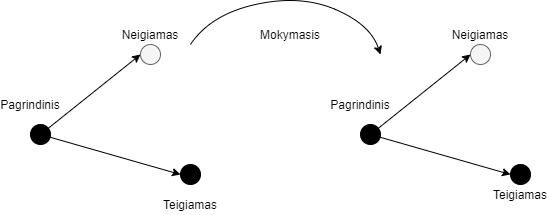
\includegraphics[scale=0.5]{img/Triplet_network}
\caption{Trejeto tinklo mokymo procesas \cite{Improved_triplet_network}} % Antraštė įterpiama po paveikslėlio
\label{img:mlp}
\end{figure}
\pagebreak

\subsubsection{Tinklo komponentai}
Kaip ir minėta prieš tai trejetų tinklų modelis įvedimo dalyje reikalauja trijų įvesčių tuo pačiu metu. Kiekvienas jų turi savo pavadinimą ir reikšmę tinkle, pagrindinis $x^a$, pozityvus $x^p$, neigiamas $x^n$. Įvesties poros $x^a$ ir $x^p$ yra tos pačios kategorijos klasės arba panašūs semantiškai įvestys. Tuo metu $x^a$ ir $x^n$ yra skirtingos kategorijos arba nepanašūs vaizdai. Pasitelkiant funkcijas yra apskaičiuojama jų semantiniai panašumai atstumo erdvėje (nes jie yra pateikiami kaip vektoriai). Ši funkcija yra vadinama nuostolių funkcija, jos viena iš galimų funkcijų yra aprašyta žemiau. Kur parametras $\alpha$ rodo semantinį tarpą tarp $x^a$ ir $x^p$ bei $x^a$ ir $x^n$. $N$ reiškia skaičių nusakantį kiek trejetų įvesčių yra pateikta. Tikslas yra pasiekti, kad $x^a$ ir $x^p$ būtų mažiau nei $x^a$ ir $x^n$ \cite{Face_recognition}.

\[loss = \sum_{x=1}^{N} max(d(x^a, x^p) - d(x^a, x^n) + \alpha, 0)\]
Kur $d$ yra atstumo metrika, taip kad $d(x^a, x^p) < d(x^a, x^n)$, o $N$ yra skaičius trejetų.

Nuostolių funkcija nusako, kaip gerai algoritmas modeliuoja pasirinktą duomenų rinkinį. Jeigu prognozė rezultatui yra netiksli, ši funkcija grąžina didesnę reikšmę. Neuroninių tinklų modeliams galima naudoti ir kitas nuostolių funkcijas, priklausomai nuo duomenų rinkinio ir norimo rezultato gauti.

\subparagraph{Alternatyvios nuostolių funkcijos}
Artima šiai funkcijai yra ši lygtis. Ji naudoja kvadratinį Euklido  \cite{Aerial_image_similarity} atstumą kaip atstumo metriką ir $\alpha > 0$, nurodanti ribą tarp dviejų vaizdų ir absoliučios sumos reikšmės.
\[loss = \sum_{x=1}^{N} [||x^a - x^p|| - ||x^a - x^n|| + \alpha]\]

\begin{figure}[H]
\centering
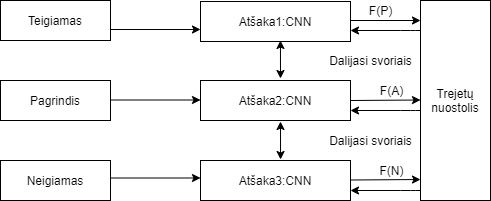
\includegraphics[scale=0.8]{img/Triplet_network_branchCNN}
\caption{Trejeto tinklų veikimo principas kartu su neuroninių tinklų lygiagrečiomis atšakomis} % Antraštė įterpiama po paveikslėlio
\label{img:mlp}
\end{figure}

Šis neuroninių tinklų architektūrinis sprendimas padeda apmokyti duomenų klasifikavimą išskaidant duomenis pagal panašumus ir skirtumus 2 pav.. Jų metu keli lygiagretūs gileiji neuroniniai tinklai yra apmokami bei tuo pačiu metu jie dalijasi svoriais vieni su kitu atlikant mokymą tinkle. Trejetų tinkle tikslas yra sukurti trejetus, kurie susideda iš pagrindinio $p^a$, teigiamio $x^p$, neigiamio $p^n$ − įvesties elementų. Pagrindinis elementas, tai kažkokia įvestis (nuotrauka, paveiksliukas, muzikos įrašas ir t.t), kuriai mes bandome rasti atitikimą iš kitos įvesties. Teigiama įvestis – panašus elementas atitinkamai pagrindiniai nuotraukai. Tuo tarpu neigiamas elementas skaitosi tas, kuris neturi panašumų su pagrindine nuotrauka. Neuroninai tinklai apskaičiuoja  $\pi : f(\pi) \in$
Šie trys elementai yra įvedami nepriklausomai vienas nuo kito į  tris identiškus giliuosius neuroninius tinklus, kurie dalijasi vienoda architektūra ir parametrais. Jų metu yra apskaičiuojami atstumai tarp šių elementų. Šiam apskaičiavimui yra naudojama kaip ir prieš tai minėta nuostolių funkcija.
\newline
Įmanomi rezultatai trjetų tinkle:
\begin{itemize}
\item{Lengvas trejatas: trejetai, kurie turi nuostolį, su reikšme 0, nes $d(x^a, x^p) + \alpha < d(x^a, x^p)$}
\item{Sudėtingas trejetas: trejetai, kurių neigiamumas yra arčiau pagrindinio negu teigiamo, $d(x^a, x^p) < d(x^a, x^p)$}
\item{Pusiau sudėtingas trejetas: trejetai, kurių neigiamumas nėra arčiau teigiamo, tačiau vis tiek turi teigiamą nuostolį: $d(x^a, x^n) < d(x^a, x^p) +\alpha$}
\end{itemize}

\subsection{Siamo tinklas}
Pirma kartą publikuotas 1990 metais, autorių Bromely ir Yann LeCun, siekiant išspręsti parašo verifikavimo problema kaip vaizdo atitikimo probelmą \cite{Siamese_signature_verifiction}.
\subsubsection{Tinklo komponentai}
Tinklo modelis – neuronų tinklas turintys kelis ar daugiau identiškus neuroninių tinkle atšakas su vienodais parameterais \cite{Siamese_Network} (panašiai kaip ir trejetų tinklų modelyje). Šis modelis naudoja vienodus svorius vykdant tuo pačiu metu ir panaudojant du skirtingus įvesties vektorius, apskaičiuojant palyginamus išvesties vektorius. Šie vienodi tinklai su skiringais įvesties duomenimis yra sujungti pagal energijos funkciją $E$. Ši matematinė funkcija apdoroja kai kurias metrikas tarp labiausiai išryškintų bruožų vaizdavimų kiekvienoje pusėje.
Parametrai tarp šių vienodų tinkle yra apriboti, kad būtų vienodi. Svorių apjungimas užtikrina, kad du labai panašūs vaizdai nebūtų tarp jų atitinkamų tinkle  atšakų išvesti labai skirtinguose erdvės lokacijose. Taip pat, reikia paminėti, kad tinklas yra simetriškas, nesvarbu kuriam iš vienodų tinklų įvesime vaizdą, visada gausime tokias pačias metrikas.
Standartinė išlaidų funkcija skirta mokymosi pavyzdžiui $(x_1, x_2)$ yra pasiūlyta Hadselio. 
\[L(W,(Y, x_1, x_2)) =  \frac{1}{2}(1 − Y )(D_w)^2 + (Y) \frac{1}{2} {max(0, m − D_w)}^2\], jei $(x_1, x_2)$  yra panašios poros, ir $Y = 1$ kitu atveju. $m$ yra riba nurodanti norimą slenkstį atstumui tarp $x_1$ ir $x_2$ jeigu jie nėra panašūs. Dėl laisvo suregualiavimo, dažniausiai taip yra sunkiau apmokyti trejetų tinklus negu Siamo tinkle. Tarkime $x_1, x_2$ yra pora vektorių, $Y$ laikysime dvejatainę žymę, kur $Y = 1$ reiškia, kad vektoriai $x_1, x_2$ yra laikomi panašiais, $Y = 0$ - priešingu atveju. $D_w$ - parametrizuota atstumo funkcija (Euklido).

\begin{figure}[H]
\centering
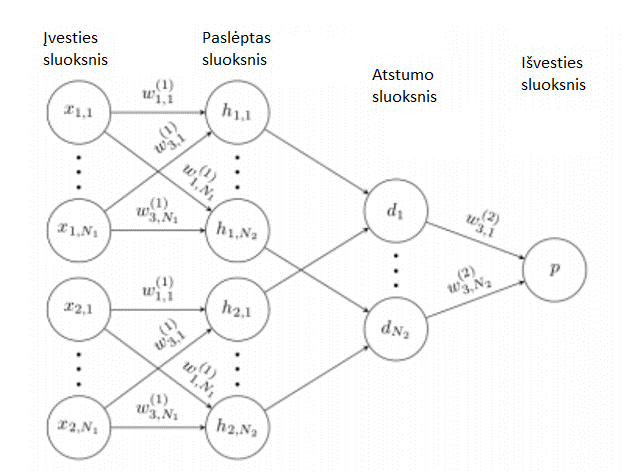
\includegraphics[scale=1.0]{img/Siamese}
\caption{Siamo tiklų modelis} % Antraštė įterpiama po paveikslėlio
\label{img:mlp}
\end{figure}

\subsection{Nefiksuoto dydžio vaizdai konvoliuciniuose tinkluose}
Gilieji konvoliuciniai tinklai reikalauja fiksuoto dydžio įvesties vaizdų. Tačiau realiame gyvenime nuotraukų ar paveiksliukų dydžiai nėra fiksuoti ir varijuoja plačiai.
\newline
Jeigu yra bandoma primiktynai pakeisti į reikiama dydį, nuotrauką karpant ar deformuojant, informacija, patalpinta nuotraukose bus prarasta. To pasekoje tikslumas nuotraukų klasifikacijos ar objektų identifikavime bus sumažintas ir nepataisomai sugadintas. Nors neuroniniuose tinkluose, konvoliuciniai sluoksniai nereikaljau fiksuoto dydžio įvesties ir geba generuoti specifinius bruožus vaizdo iš bet kokio dydžio nuotraukų. Visgi, pilnai sujungti sluoksniai privalo turėti fiksuoto dydžio įvestį dėl jų pačių apibrėžimo. Dėl to apribojimas fiksuoto dydžio nuotraukų ateina tik iš pilnai sujungtų sluoksnių reikiamos ypatybės.
Viena iš šios problemos sprendimo būdų yra naudoti erdvinės piramidės talpinimą \cite{Spatial_pyramid_pooling}, tokiu būdų galima bandyti identifikuoti vaizdus, kurių rezoliucijos yra skirtingos.
\newline
Šis būdas ištraukia vaizdo bruožus iš bruožų žemėlapio (angl. \textit{map}) per $4 x 4$, $2 x 2$ ir $1 x 1$ kvadratų tinklelio. Tada SPP sluoksnis pateikia $16 + 4 + 1 = 21$ skirtingus aruodus (angl. \textit{bin}) ir gauna fiksuoto dydžio išvestį kviečiant kviekvieną bloką. Po erdvinės piramidės talpinimo būdo išgavimo, bet kuris bruožų žemėlapis gali generuoti 5736 dimensijų ypatybių vektorius, kur $5736 = 24 x 26$. SPP sluoksnis pasiima ypatybes ir generuoja  fiksuoto dydžio išvestis, kuris galiausiai yra perduodamas į pilnai sujungtus sluoksnius.
\pagebreak

\section{Įvertinimo funkcija}
Kelios įvertinimų metrikos yra naudojamos: panašumo tikslumas bei \emph{score-at-top-K}, kai $K = 30$. Panašumo tikslumas yra išreiškiamas procentaliai pagal tai, kiek trejetų buvo korektiškai sureitinguota. Sakykime, kad turime trejetą, su šiais įvesties parametrais $tt = (x^a, x^p, x^n)$, kur $x^p$ turėtų būti arčiau(panašesnis)šalia $x^a$. Laikant, kad $x^a$ yra įvesties užklaus,a žiūrime į rezultatus kitų įvesties duomenų. Jeigu $x^p$ yra reitinguojamas aukščiau nei $x^n$, tai tada teigiame, kad atitinkamas trejetas yra sureitinguotas teisingai. Kita mums reikalinga metrika, kuri buvo užsiminta anksčiau \emph{score-at-top-K}. Jis nusako skaičių teisingai sureitinguotų trejetų bei atimant iš jo skaičių, kuris nusako neteisingai sureitinguotus trejetus iš pogrupio trejetų, kurių reitingas yra didesnis, nei kintamasis $K$. Pogrupis yra pasirenkamas tokia tvarka: kiekvienam užklausos paveikslėliui iš duomenų aibės, ištraukia 1000 naujų paveikslėlių iš tos pačios teksto užklausos ir yra bandoma taip reitinguoti juos, pasitelkiant išmoktas metrikas. Jei trejetų reitingas yra aukštesnis negu $K$, jeigu jo $x^p$ arba $x^n$ tada yra tarp geriausiai reitinguojamų $K$ kaimynų iš užklausos su paveikslėliais $x^a$.
\pagebreak

\subsection{Asmens pakartotinis identifikavimas}
Pastaraisias metais asmens pakartonis identifikavimas, naudojant kompiuterinį mokymą pritraukia vis daugiau dėmesio. Klestint giliajam mokymui yra sukuriama daugiau skirtingų modelių norint pasiekti šį tikslą(asmens identifikavimas). Vienas iš modelių, susilaukusių labai daug dėmesio yra FaceNet, šis konvoliucinis tinklas yra taikomas apmokyti bruožų įterpimą veidams atpažinti.

\subsection{Pasirenkami duomenis įvertinimui analizuoti}
Kadangi darbo tema susijusi su detaliu vaizdų atpažinimuu, kuris negali būti charakterizuotas pagal vaizdų kategorijų žymes, literatūroje buvo surasta informacijos, panaudojant trejetų duomenų rinkinys norint įvertinti nuotraukų panašumus su skirtingais modeliams \cite{Learning_fine_grained_image}.
Buvo paimta 1000 populiariausių teksto užklausų su atrinktais trejetais $(x^a, x^p, x^n)$ su Google 50 paieškos rezultatų kiekvienai užklausai \cite{Learning_fine_grained_image}.

Atpažinimo efektyvumas pagal metrikas yra nurodytas 1 lentelė ir 2 lentelė. "DeepRanking", kuris  paminėtas buvo literatūroej, yra gilusis reitingavimo modelis mokomas su 20\% neigiamais pavyzdžiais. Visgi pastebima, kad joks vaizdų atpažinimo modelis be mokymo nepasiekia gerų rezultatų ir nėra dinamiškai prisitaikantys prie naujo duomenų rinkinio, kuris priklauso kitoms vaizdų klasifikacijos kategerijoms. L1HashKCPA pasiekė visai neblogą rezultatą su ganėtinai mažai dimensijų, tačiau jo našumas yra ganėtinai prastesnis negu "DeepRanking" metodo.
\pagebreak
\begin{center}
\begin{tabular}{ | m{10em} | m{5em}| m {3em} |} 
\hline
Metodas & Tikslumas & Score-30 \\
\hline
ConvNet & 82.8\% & 5772 \\
\hline
Single-scare Ranking & 84.6\% & 6245 \\
\hline
OASIS on Single-scale Ranking & 82.5\%  & 6263 \\
\hline
Single-Scale $\&$ Visual Feature & 84.1\% & 6765 \\
\hline
DeepRanking & 85.7\% & 7004\\
\hline
\end{tabular}
\captionof{table}{Tikslumo metrikų rezultatai (1)}
\end{center}

\begin{center}
\begin{tabular}{ | m{10em} | m{5em}| m {3em} |} 
\hline
Metodas & Tikslumas & Score-30 \\
\hline
Wavelet & 62.2\% & 2735\\
\hline
Color & 62.3\% & 2935 \\
\hline
SIFT-like & 65.5\%  & 2863 \\
\hline
Fisher $\&$ Visual Feature & 67.2\% & 3064\\
\hline
HOG & 85.7\% & 7004\\
\hline
SPMKtexton1024max & 66.5\% & 3556\\
\hline
L1HashKPCA & 76.2\% & 6356\\
\hline
OASIS & 79.2\% & 6813\\
\hline
Golden Features & 80.3\% & 7165 \\
\hline
DeepRanking & 85.7\% & 7004\\
\hline
\end{tabular}
\captionof{table}{Tikslumo metrikų rezultatai (2)}
\end{center}

\pagebreak

\section{Trejetų tinklo vaizdų atpažinimo tyrimas ir vertinimas}
\subsection{Tikslumo metrikos}
Šiame darbe buvo naudojama tikslumo metrika (4), kuri nauodojoma dvejatainių klasifikatorių vertinime.

\[ accuracy=\frac{\sum  \ \ \textrm{Teigiamas} + \sum \ \ \textrm{Neigiamas} }{\sum \ \ \textrm{Visa populiacija} } \]

Kadangi yra labai retas atvejis, kad $d(x_a, x_p)$ būtų lygus $d(x_a, x_n)$, galima laikyti, kad $\sum \ \ \textrm{Teigiamas}$ tai yra lygu $\sum \ \ \textrm{Neigiamas}$. Del to, būtų galima skaičiuoti tik $\sum \ \ \textrm{Teigiamas}$ iš visų įvesties trejetų sumos $N_t$ mokomojame rinkinyje. Galutinė lygtis (5), kuri naudojama tikslumui lyginti.
\[ accuracy=\frac{\sum d(x_a, x_p) + \sum d(x_a, x_n) }{ N_t } \]

\subsection{Apmokymo ir testavimo aplinka}
Trejetų tinklo modelis buvo apmokmamas naudojant  savo personalinį Lenovo Y-700 kompiuterį su turimomis šiomis specifikacijomis: CPU I7-6700K keturių  branduolių, GPU Nvidia GeForce GTX 960M (4GB RAM). Kompiuteryje yra naudojama 8 GB
dydžio operatyvioji atmintis. Taip pat bandymų aplinkoje buvo įdiegta Windows 10 operacinė sistema. Norint pasileisti trejetų modelį būtent šiam kompiuteriui (priklausomai nuo mašinos tai gali skirtis) buvo atsisiųsta Nvidia CUDA programinė įranga su tikslu, kad modelio mokymas bus vykdomas pasitelkiant vaizdo plokštę, o ne procesorių.
\newline
Priežastis kodėl buvo pasirinkta vaizdo plokštė yra todėl, kad gilusis mokymasis yra intensyvi skaičiavimo užduotis. Į gilųjį mokymasi įeina didžiuliai matricų skaičiavimai (ypač sandauga) ir kitos operacijos, kurios gali veikti paraleliai todėl vaizdo plokštė ateina į pagalbą, nes viena vaizdo plokštė gali turėti tūkstančius branduolių, tuo metu procesorius turi žymiai mažiau branduolių, nors jie ir žymiai greitesni negu vaizdo plokštės \cite{Performance_of_GPU}.
\newline
Pasirenktas trejetų tinklų modelis yra įgyvendintas naudojant Tensorflow karkasą su Python 3.5.1 versija.
\newline
Vaizdų duomenų rinkinyje buvo 3884 nuotraukos, kuriose jau buvo surikiuotos teisinga eilės tvarka, kur pirma nuotrauka pagrindinė, antra nuotrauka - teigiama (kuri yra panaši į pagrindinę) bei neigiama (nepanaši į pagrindinę nuotrauką) ir tokia eilės tvarka yra išsidėstę visos kitos nuotraukos.
Apmokius, naudojant šiuos duomenis, yra bandoma analizuoti modelio tikslumą imant vaizdų pavyzdžius iš testinio duomenų rinkinio.

\subsection{VGG16 tinklo modelis}
VGG16 yra konvoliucinių neuroninių tinklų modelis, išrastas K. Simonian ir A. Zisserman (Oksfordo universitetas). Modelis sugeba pasiekti 92.7\% top-5 testų tikslumą (mokymo duomenys pasiimti iš ImageNet). VGG16 buvo mokomas savaitę iš savaitės naudojant Nvidia Titan Black vaizdo plokščių šeimas.
Šiame darbe, žmonių siluetų atpažinimui yra naudojamas trjetų tinklų modelis \cite{Aerial_image_similarity}. Modelis naudoja modifikuota nuostolių funkciją: 
\[loss = \sum_{i+1}^{N_t} [\ln ( - \frac{\sum_{j=1}^{N} (f_o^a - f_o^p)^2 }{\beta} + 1 + \epsilon) + \ln(- \frac{\sum_{j=1}^{N} (f_o^a - f_o^n)^2}{\beta} + 1 + \epsilon)  ] \]


Kur $f_o^a$ yra ModelNN išvestis pagrindiniai nuotraukai, $f_o^p$ ir $f_o^n$ yra ModelNN išvestys teigiamai ir neigiamai nuotraukoms. $N$ yra išvesties vektoriaus dimensijos, o  trejetų skaičius mokymo duomenų rinkinyje. $\epsilon$ yra koks nors mažas skaičius, pvz.: $10^-6$. Nuostolių funkcija yra 0, kai teigiama ir neigiama įvestys yra maksimaliu atstumu viena nuo kitos.  
Šio modelio architektūra klasifikavimui naudoja VGG16 tinklo bazinius sluoksnius išskyrus paskutinį sluoksnį, todėl tik labai panašūs vaizdai gali būti naudojami duomenų mokymui tam, kad pagerinti tinklo atlikimą bei išsaugoti skaičiavimo išteklius. Vietoj paskutinio tinklo modelio buvo pasirinktas, naudoti pagal pasirinktą šaltinį VALAICIO, modifikuotas apmokamas sluoksnis.
Tinklas apdoroja vaizdo įterpimus, kurie vėliau yra atgaunami iš paskutinio sluoksnio.
\begin{figure}[H]
\centering
\includegraphics[scale=0.6]{img/CustomVGG16}
\caption{Naudojamo tinko modelis} % Antraštė įterpiama po paveikslėlio
\label{img:mlp}
\end{figure}

Modifikuoti tinklo sluoksniai susideda iš vieno pilnai sujungto sluoksnio, kurio dydis yra 28x28x1 bei išlyginimo sluoksnis, kuris yra skirtas gauti vektorių, kad suskaičiuoti trejetų nuostolį.
Taip pat buvo naudojamas Adam optimizavimo metodas. Šis metodas buvo pasitinktas, nes jis fiksuoja vienus geriausius rezultatų. Kartu su juo buvo naudoti hyperparametrai, kurie apmokymo metu buvo koreguojami norint gauti geriausius rezultatus. Išbandžius daug skirtingų varijacijų su hiperparametrais, geriausi rezultatai buvo finksuoti su tokiomis reikšmėmis:  (= 10−3, β1 = 0.9, β2 = 0.999). Aktyvacijos funkcijai buvo pasirinkta Sigmoidinė funkcija, priešingai nei tiesinė funkcija, ji sugeba susitvarkyti gerai su komplikuotais duomenų rinkiniais.

\subsection{Tyrimo rezultatai}
Buvo parinkti mokymui keli skirtingi duomenų rinkiniai: CUHK01 ir  Market-150. Pastarasis duomenų rinkinys duomenų kiekiu buvo didžiausias. Jis laiko 32668 vaizdus iš 1501 skirtingų asmenų identifikacijų. Šie duomenys yra išskaidyti  į apmokamų ir testuojamų vaizdų rinkinius atitikamai 12936 ir 19732.
Kdangi tinklas naudoja tris lygiagrečias įvestis buvo labai svarbu užtikrinti, kad pagrindinės nuotraukos būtų panašios į teigiamas nuotraukas, o neigiamos nuotraukos, būtų nepanašios. Klaidos atveju tinklas prastai parinkdavo svorius dėl to prasti rezultatai būdavo fiksuojami.
Kad naudotis šiais duomenų rinkiniais specialus duomenų rinkinys buvo sukurtas, kuris susidejo iš skirtingų trejetų vaizdų. Pagrindinė ir pozityvi nuotraukos priklauso tam pačiam asmeniui, tačiau šis asmuo būdavo fiksuojamas iš skirtingų momentų, todėl minimaliai skirdavos šios nuotraukos. Neigiamoms nuotraukoms buvo atsitikine tvarka parenkami žmonių siluetai. Įvesties dimensijos VGG16 tinklui yra 224x224 todėl trejetams būdvo pakeičiamas dimensijų dysis į šį.
Vienas iš duomenų rinkinių atpažinti detalius vaizdus, naudojant vaizdų duomenų rinkinį CUHK01. Šiame duomenų rinkinyje yra pavaizduota 3884 viešose vietose einančių pėsčiųjų kadrai. Todėl naudojant ši duomenų rinkinį buvo analizuojama, kaip su pasirinktu trejetų modeliu seksis atpažinti skirtingus žmogaus kadrus, kurie buvo nufotografuoti įvairiai -  iš kelių pusių, iš nugaros ir priekio, esant skiringai žmogaus eisenos pozicijai, skirtingam apšvietimui ir kontrastamas, įsiterpiant kitiems objektams prie pėsčiojo.
\newline
Apmokius trejetų tinklą su pasirinktu duomenų rinkiniu ir pradėjus testuoti jo rezultatus, gavau 85,7\% tikslumo rezultatą. Tai yra gan aukštas įvertinimas, nes atpažinti to paties pėsčiojo skirtingus kadras nėra lengviausia užduotis, nes susiduriame su kliūtimis, aprašytomis anksčiau. Jeigu palyginsime kaip sekėsi kitiems neuroninių tinklų modeliams atpažinti būtent šį duomenų rinkinį, turime tokius rezultatus:
90.4\% , kur neuronų tinklų modelį sukūrė mokslininkai iš Kinijos Mokslų ir Technologijų universiteto. \cite{Person_reindentification}
\begin{figure}[H]
\centering
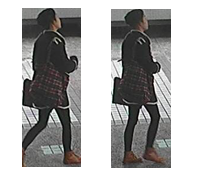
\includegraphics[scale=1.0]{img/Frame_diff.png}
\caption{Žmogaus skiringi eisenos kadrai} % Antraštė įterpiama po paveikslėlio
\label{img:mlp}
\end{figure}
Taip pat, žemiau pateikiu kitus rezultatus, gautus su kitais neuroniais tinklų modeliais:

\begin{center}
\begin{tabular}{ | m{7em} | m{5em}| } 
\hline
Modelis & Tikslumas \\
\hline
Spindle & 94.4\% \\
\hline
PSE & 86.6\% \\
\hline
Part-Aligned& 94.4\% \\
\hline
AACN & 96.7\% \\
\hline
\end{tabular}
\captionof{table}{CUHK01 duomenų tikslumo rezultatai}
\end{center}

\pagebreak

\subsection{Vaizdai su prastais rezultatų palyginimais}
Visgi ne visi vaizdai buvo tesingai palyginimi ir nustatomi trejetų tinklo modelio. Todėl šiame darbe buvo ieškoma ir nagrinėjama, kurios vaizdų įvestis turėdavo prastus rezultatus bei buvo bandoma išsiaiškinti kas sukeldavo prastus rezultatus.

\begin{figure}[H]
\centering
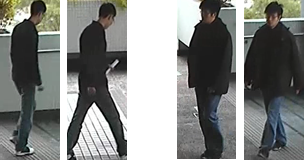
\includegraphics[scale=1.0]{img/Wrongly_detected.png}
\caption{Blogai identifikuotos vaizdų poros} % Antraštė įterpiama po paveikslėlio
\label{img:mlp}
\end{figure}

Dauguma nuotraukų, kurios buvo blogai identifikuotos skirėsi viena nuo kitos spalvų intensivumu, skirtingomis spalvomis. Pavyzdžiui matome, kad tiek pirmoje ir antroje nuotraukų porose įsiterpusi nauja žalia spalva (žalumos objektai) leidžia manyti, kad tai yra viena iš priežasčių, kodėl nepavyko tinkamai identifikuoti to paties asmens kadrus. Taip pat antroje poroje matome, kad žmogaus judėjimo kampas į objektyvą skiriasi, o ir nuotraukų šviesos intensyvumas yra kitoks. Todėl tai leidžia daryti prielaida, kad ir vaizdų palyginimo rezultatai bus prasti, jei nuotraukos bus nufotografuotos ne kokybiškai - apšvietimo skirtumai, netvarkingas fonas ar atsiradusi okliuzija \cite{Person_reindentification}.
\pagebreak

\begin{figure}[H]
\centering
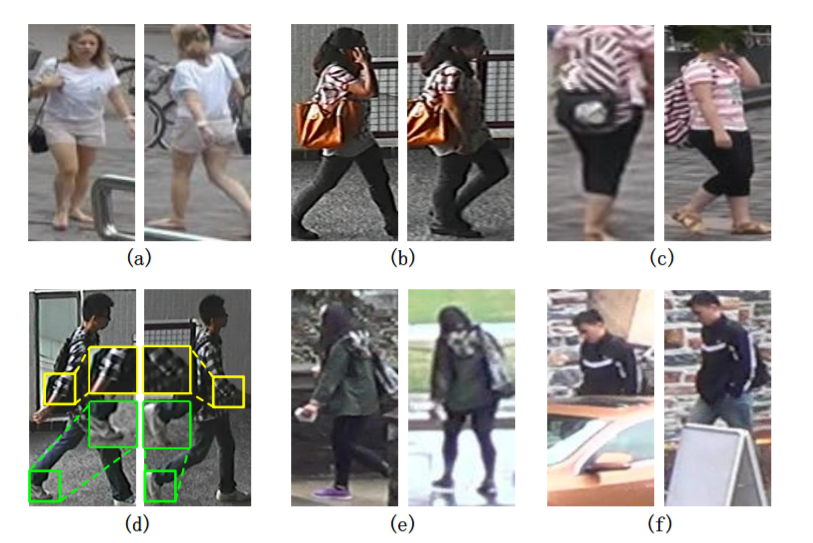
\includegraphics[scale=1.0]{img/image_diff_examples.png}
\caption{Sunkiai identifikuojamų nuotraukų poros} % Antraštė įterpiama po paveikslėlio
\label{img:mlp}
\end{figure}
Viršuje esančios žmonių nuotraukų poros yra sudėtingai identifikuojamos dėl įvairių priežasčių: a) dėl skirtngo objektyvo kampo, b) skirtingos žmogaus pozos, c) prastos nuotraukos kadro užfiksavimo (susiliejas vaizdas), d) ne vienodame lygyje esančios žmogaus kūno dalis, atsiradusios dėl jo judėjimo, e) netvarkingas fonas, f) okliuzija.

\subsection{Sprendimo būdai}
Visgi ieškant literatūroje informacijos, kurioje būtų aprašyti sprendimo būdai, kai lyginami vaizdai vienas su kitu yra nekorektiški bruožų atžvilgiu, tačiau panašūs ar priklauso tai pačiai klasei, yra siūlomi keli sprendimų būdai. Pavyzdžiui, ypatybių fokusavimą nukreipiant į lokalias detales buvo sukurtas nesudėtingas suskirstymas asmens nuotraukos į kelias fiksuotas ir nekintančias dalis, pavyzdžiui į horizontales juosteles ir taip mokantis lokalių nuotraukų bruožų atpažinimo. Visgi, kaip tyrimai iš literatūros nurodė toks skirstymas prastai lygina identifikuojamo asmens kūno dalis \cite{Person_reindentification}. Kituose tyrimuose ir bandymuose buvo bandoma naudoti žmogaus pozą, tokiu būdu identifikuojant skirtingas kūno dalis: kojas, rankas, veidą. Tačiau ir toks atpažinimo metodas yra prastas, kad gauti norimus rezultatus, nes identifiuoti tas pačias žmogaus kūno dalis iš skirtingų žmogaus padėčių kelia problemų dėl asmens skirtingos judėjimo pozos nuotraukos \cite{Person_reindentification}.
\pagebreak
\section{Rezultatai ir išvados}
\thispagestyle{empty} 
\subsection{Rezultatai}
\begin{enumerate}
\item{Buvo lyginimi kiti trejetų tinklai rinkoje, nagrinėjami jų rezultatai.}
\item{Buvo pasiūlytas trejetų tinklų modelis, kuris sugebėjo teisingai atpažinti 85.7\% vaizdų, palyginus su kitais rinkoje esančiai modeliais, kurių rezultatai sviruoja nuo 86.6\% iki 96.7\%, pasirinktas modelis turėjo konkuruojančius rezultatus, nors ir ne pačius geriausius.}
\item{Buvo išskirtos metrikos pagal ką reitinguoti vaizdų atpažinimą.}
\item{Aprašyti tyrimo rezultatai, rastos problemos, dėl kurių yra sudėtinga labai gerai atpažinti nuotraukos, viena iš priežasčių, žmogaus eisenos trajetorijos skirtumai tarp lyginamų vaizdų.}
\end{enumerate}
\subsection{Išvados}
\begin{enumerate}
\item{Yra sudėtinga lyginti trejetų ir Siamo modelius, nes jų architektūra gali varijuota pagal tai kaip modelis yra įgyvendintas. Teisingiau yra lyginti specialius jų sukurtus modelius vienas su kitu.}
\item{Pasirinktas trejetų tinklų modelis parodė neblogus rezultatus identifikuojant žmonių eisenos kadrus.}
\item{Identifikuojant žmones nuotraukose susiduriama su rimtomis problemomis, kai to paties žmogaus nuotraukos skiriasi dėl pašalinių priežasčių. Kas lemia kad žmonių identifikacija yra sudėtingas procesas, kuris tam tikroms nuotraukoms neturi sprendimo būdų.}
\end{enumerate}
\subsection{Ateities darbai}
\begin{enumerate}
\item{Išbandyti kitą trejetų modelį su pasiūlytais būdais, kurie gebėtų dar geriau atpažinti žmonių siluetus}
\item{Atlikti atpažinimo rezultatų analizę su kitis neuronų tinklais.}
\item{Ištestuoti su daugiau duomenų rinkinių. Stebėti ir lyginti rezultatus}
\item{Iškelti savo palyginimo metodą, kuris gebėtų teisingai identifikuoti žmonių siluetus nuotraukose.}
\end{enumerate}
\pagebreak

\section{Priedai}
\thispagestyle{empty} 
\subsection{Žodynas}
\begin{itemize}
\item{Svoris(angl. \textit{weight}) - parametras neuroniname tinkle, kuris transformuoja įvesties duomenys paslėptuose sluoksniuose.}
\item{Nuostolių funkcija(angl. \textit{loss function}) - funkcija, padedanti optimizuoti svorius, taip sumažinant neatitikimų nuostolius.}
\item{Detalieji vaizdai(angl. \textit{fine-grained}) - detalūs vaizdai. Vaizdo klasifikavimo užduotyse, tai yra įvesties vaizdai, kuriuos yra sudėtinga išskirti klasėms, pvz.: identifikuojant skirtingų markių automobilius.}
\item{Aktyvacijos funkcija(angl. \textit{activation function}) - funkcija, skirta nustatyti ar neuronas turi būti aktyvuotas, skaičiuojant svorių sumą bei pridedant postūmio parametrą.}
\item{Postūmis(angl. \textit{bias}) - papildomas parametras neuroniniuose tinkluose, kuris padeda koreguoti išvesti kartu su svorių įvesties suma, skirta neuronams perduoti. Taip pat šis parametras leidžia perstūmti aktyvacijos sumą nuo kairės į dešinę.}
\end{itemize} 
\pagebreak

\printbibliography[heading=bibintoc] 
\thispagestyle{empty}

\end{document}

